% =====================================================================
%  PRL letter: one kinetic flow rule for plasticity, strain-rate
%  sensitivity and creep of BCC metals and alloys
%  Compile: pdflatex main && bibtex-free (references inline) -> pdflatex main
%  Figures: ./figures/fig2_srs.pdf, fig3_lambda.pdf, fig4_maps_creep.pdf
%  Items marked \todo{} must be checked before submission.
% =====================================================================
\documentclass[aps,prl,twocolumn,superscriptaddress,amsmath,amssymb,floatfix]{revtex4-2}

\usepackage{graphicx}
\usepackage{bm}
\usepackage{xcolor}
\usepackage{tikz}
\usetikzlibrary{arrows.meta,positioning,fit,calc}
\usepackage[colorlinks=true,citecolor=blue!50!black,linkcolor=blue!50!black,urlcolor=blue!50!black]{hyperref}

\newcommand{\gd}{\dot\gamma}
\newcommand{\ts}{\tau^{\star}}
\newcommand{\kT}{k_BT}
\newcommand{\todo}[1]{\textcolor{red}{[#1]}}
\newcommand{\fig}[2]{\IfFileExists{figures/#1}{\includegraphics[width=#2]{figures/#1}}{\fbox{\parbox[c][3cm][c]{#2}{\centering figures/#1}}}}

\begin{document}

\title{Time-additive dislocation kinetics unify strain-rate sensitivity, dynamic strain aging and creep in body-centered-cubic metals}

\author{Matthew Maron}
\affiliation{\todo{Affiliation}}
\author{Giacomo Po}
\affiliation{\todo{Affiliation}}
\author{Yang Li}
\affiliation{\todo{Affiliation}}

\date{\today}

\begin{abstract}
The strain-rate sensitivity $m$ is widely used to diagnose changes in the rate-controlling mechanism of plastic flow. Yet non-monotonic $m(T)$, negative $m$, and the transition from plasticity to creep are usually described with separate laws joined by phenomenological onset functions. We show that one flow rule, built from the \emph{time} a dislocation segment spends per obstacle spacing, captures all of these regimes. Sequential processes add their times, alternative bypass routes add their rates, and simultaneous resistances add their stresses. Because solute aging is fixed by the imposed rate, the flow stress is unique even where $m<0$. Differentiating the flow rule gives an exact decomposition, $1/m=\tau A/(1+AB)$, into an intrinsic mobility sensitivity $A$ and a rate-sensitive resistance $B$, with $m<0$ exactly when $AB<-1$. With material-specific microstructure but no switching functions, the same rule describes the flow stress, $m$ and activation volume of W, Zr and Eurofer-97, and the minimum creep rates of Eurofer-97 over four orders of magnitude.
\end{abstract}

\maketitle

% ---------------------------------------------------------------------
\paragraph{Introduction.}
Plastic flow of body-centered-cubic (BCC) metals, and prismatic slip in hexagonal Zr and Ti, is controlled at low temperature by thermally activated kink-pair nucleation on screw dislocations~\cite{HirthLothe,Po2016}. As temperature increases, the flow stress drops onto an athermal plateau. It then shows dynamic strain aging (DSA) humps~\cite{Cheng2001,KubinEstrin1990}, and finally falls steeply as diffusion-assisted recovery and climb take over~\cite{FrostAshby}. The strain-rate sensitivity $m=\partial\ln\tau/\partial\ln\gd$ and the apparent activation volume $V^\star=\kT/(m\tau)$ are the standard experimental probes of these transitions. They are also the quantities crystal-plasticity and finite-element (FE) models need for rate- and temperature-dependent structural analysis.

Constitutive descriptions usually take one of two routes. Either stresses are added, $\tau=\tau_a+\ts+\tau_d$~\cite{Seeger,KocksArgonAshby,EstrinMcCormick}, or the rates of independent mechanisms are added~\cite{FrostAshby}. Neither route alone gives the ordering of processes a moving dislocation actually experiences. In practice, regime changes are imposed with sigmoidal onset functions in temperature or grain size. As a result, a non-monotonic $m(T)$ is often read as a change of mechanism even when none occurs.

We propose a single flow rule in which regime changes follow from the kinetics. We apply it without modification to a pure refractory metal (W), a hexagonal metal with strong oxygen aging (Zr), and a precipitate-strengthened fusion steel (Eurofer-97). The same rule covers tensile tests from $10^{-5}$ to $10^{-1}$~s$^{-1}$ and creep down to $10^{-10}$~s$^{-1}$.

% ---------------------------------------------------------------------
\paragraph{Flow rule.}
The Orowan relation $\gd=\rho_m b\bar v$ is written with the mean velocity $\bar v=\lambda/(t_r+t_w)$. Here $t_r$ is the time a segment spends \emph{travelling} between obstacles of spacing $\lambda$ and $t_w$ is the time it spends \emph{waiting} at them. Three composition rules follow (Fig.~\ref{fig:scheme}).
\begin{enumerate}
  \item[(S)] Processes that one segment passes through in sequence add their times, $\gd^{-1}=\sum_i\gd_i^{-1}$.
  \item[(P)] Alternative routes past the same obstacle add their rates, $\nu_j=\sum_k\nu_{jk}$.
  \item[(L)] Resistances that act simultaneously along the line add their stresses, as in Kocks' linear superposition of dense-weak and sparse-strong obstacles~\cite{KocksArgonAshby}.
\end{enumerate}
The result is
\begin{align}
\frac{1}{\gd}&=\frac{1}{\rho_m b\,v_g(\ts)}+\frac{1}{\rho_m b}\sum_j\frac{n_j}{\sum_k\nu_{jk}(\ts)},\label{eq:flow}\\
\tau&=\tau_a(\bm s)+\ts+\sum_g\tau_g(\gd),\label{eq:tau}
\end{align}
where $n_j$ is the number of type-$j$ obstacles met per unit glide distance, $\bm s$ is the microstructural state, and $\tau_g$ are the stresses of superposed obstacle groups, each solved from its own waiting kinetics.

The travel velocity $v_g$ is the kink-pair law of Ref.~\cite{Po2016},
$v_g=(\ts b/B)\exp\{-\Delta H_0[(1-(\ts/\tau_P)^p)^q-T/T_0]/2\kT\}$,
with the factor $1/2$ from the long-segment regime. The bypass routes are:
\begin{itemize}
  \item thermal cutting or detachment, $\nu=\nu_0\exp\{-F[1-(\ts/\hat\tau)^p]^q/\kT\}$, which becomes the Orowan limit when $\ts\geq\hat\tau$;
  \item glide-assisted climb, $\nu=v_c/h$ with $v_c\propto D\,[e^{\ts\Omega/\kT}-1]$.
\end{itemize}
The athermal stress is Taylor-type, $\tau_a=\alpha\mu b(\sqrt{\rho}+\Lambda_b)$, with $\rho$ from Kocks--Mecking kinetics~\cite{MeckingKocks} extended by climb-controlled recovery,
\begin{equation}
\frac{d\rho}{d\gamma}=k_1(\sqrt\rho+\Lambda_b)-k_2\rho-\frac{K_{cl}D(T)}{\gd}\rho^2.
\label{eq:km}
\end{equation}
The last term gives the $n=3$ natural creep law when it dominates.

Solutes segregate to waiting segments~\cite{CottrellBilby,Louat1981,Cheng2001}:
\begin{equation}
\frac{C}{C_0}=1+\sum_iC_i\left[1-e^{-(t_a/t_{D,i})^{\alpha_i}}\right],\qquad t_a=\frac{\rho_m b\lambda}{\gd},
\label{eq:aging}
\end{equation}
which strengthens the pinning by a factor $\sqrt{C/C_0}$. Diffusional (Nabarro--Herring and Coble) flow is an independent carrier, so its rate is added to Eq.~(\ref{eq:flow}).

Because every state variable in Eqs.~(\ref{eq:km})--(\ref{eq:aging}) depends on $(\gd,T,\gamma)$ but not on $\tau$, the right-hand side of Eq.~(\ref{eq:flow}) is strictly monotonic in $\ts$. For any imposed rate the stress is therefore unique, including where DSA makes $\tau(\gd)$ decrease. No onset function appears anywhere. The ``switches'' are the time fractions $w_i=\gd/\gd_i$ of the sequential steps and the rate fractions $\nu_{jk}/\nu_j$ of the parallel routes, and both follow from activation energies, diffusivities and spacings.

\begin{figure}[t]
\centering
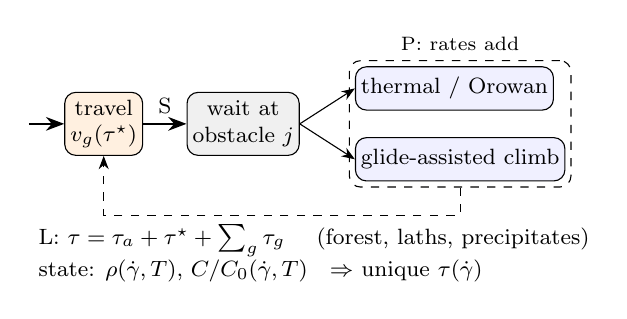
\begin{tikzpicture}[font=\footnotesize,
  box/.style={draw,rounded corners,minimum height=0.8cm,align=center,inner sep=2pt},
  rt/.style={draw,rounded corners,minimum height=0.55cm,align=center,fill=blue!6,inner sep=2pt},>=Stealth]
  \node[box,fill=orange!12] (g) {travel\\$v_g(\ts)$};
  \node[box,fill=gray!12,right=0.55cm of g] (w) {wait at\\obstacle $j$};
  \node[rt,right=0.7cm of w,yshift=0.45cm] (a) {thermal / Orowan};
  \node[rt,right=0.7cm of w,yshift=-0.45cm] (c) {glide-assisted climb};
  \draw[->,thick] ($(g.west)+(-0.45,0)$) -- (g);
  \draw[->,thick] (g) -- node[above]{S} (w);
  \draw[->] (w.east) -- (a.west); \draw[->] (w.east) -- (c.west);
  \node[draw,dashed,rounded corners,fit=(a)(c),inner sep=2pt,label={[font=\scriptsize]above:P: rates add}] (pb) {};
  \draw[->,dashed] (pb.south) -- ++(0,-0.35) -| (g.south);
  \node[align=left,anchor=north west] at ($(g.south west)+(-0.45,-0.75)$)
   {L: $\tau=\tau_a+\ts+\sum_g\tau_g$ \quad (forest, laths, precipitates)\\
    state: $\rho(\gd,T)$, $C/C_0(\gd,T)$ \; $\Rightarrow$ unique $\tau(\gd)$};
\end{tikzpicture}
\caption{The three composition rules. Travel and waiting are sequential, so their times add (S). The routes past an obstacle are alternatives, so their rates add (P). Simultaneous line resistances add their stresses (L). The state depends on the imposed rate but not on the stress.}
\label{fig:scheme}
\end{figure}

% ---------------------------------------------------------------------
\paragraph{Exact rate-sensitivity decomposition.}
Write the intrinsic mobility process (travel plus intragranular obstacles) as $\gd=G_{\rm int}(\tau^\star_{\rm int};\bm s)$ and let everything else contribute to $\tau$ through state variables or superposed groups. Differentiating Eqs.~(\ref{eq:flow})--(\ref{eq:tau}) with respect to $\ln\gd$ gives the exact result
\begin{equation}
\frac1m=\frac{\tau A}{1+\Lambda},\quad
A=\frac{\partial\ln G_{\rm int}}{\partial\ts},\quad
B=\frac{d\tau}{d\ln\gd}-\frac1A,\quad
\Lambda=AB.
\label{eq:srs}
\end{equation}
Here $A$ is the intrinsic mobility sensitivity. With the time weights of rule S it is $A=\sum_iw_iA_i$ for the sequential steps and $A_j=\sum_k(\nu_{jk}/\nu_j)A_{jk}$ for the routes past obstacle $j$. $B$ is the rate sensitivity of the resistance; it collects rate-dependent state and superposed groups. Equation~(\ref{eq:srs}) has two limits:
\begin{itemize}
  \item mobility control ($|\Lambda|\ll1$): $V^\star\to\kT A$, which increases as the kink-pair barrier softens;
  \item resistance control ($\Lambda\gg1$): $V^\star\to\kT/B$, which decreases as $B$ grows.
\end{itemize}
A peak in $V^\star(T)$ therefore signals a change from $A$-control to $B$-control, whereas a non-monotonic $m(T)$ alone does not. Solute aging makes $G$ \emph{increase} with $\gd$ at fixed stress, because faster flow leaves less time to age. Hence $B<0$, and
\begin{equation}
m<0\iff\Lambda<-1 .
\end{equation}
Negative rate sensitivity, the precondition for serrated (Portevin--Le Chatelier) flow~\cite{McCormick1988}, is thus not a separate regime but a region of the same competition map. Climb-controlled recovery and precipitate climb both give $B>0$. We checked Eq.~(\ref{eq:srs}) against finite differences of the solved stress for all three materials, including points with $m<0$; the two agree to better than $10^{-5}$.

% ---------------------------------------------------------------------
\paragraph{Tungsten.}
In W the waiting steps and the rate-dependent state are negligible below $\sim0.25T_m$, so $\Lambda\equiv0$ [Fig.~\ref{fig:lambda}]. The rise and fall of $m(T)$ [Fig.~\ref{fig:srs}(b)] then comes entirely from the kink-pair sensitivity $A$ and the athermal share $\tau_a/\tau$. As $\ts\to0$, $m\sim\ts/\tau\to0$ even though $A$ diverges. Correspondingly, $V^\star=\kT A$ rises monotonically with temperature [Fig.~\ref{fig:srs}(c)]. This behaviour is shared by micropillar, nanoindentation, plate and arc-melted W~\cite{Wdata}, although their $m(T)$ curves look qualitatively different. The CRSS data are reproduced with the mobility parameters of Ref.~\cite{Po2016}-type laws ($\Delta H_0=2.4$~eV, $\tau_P=0.8$~GPa) [Fig.~\ref{fig:srs}(a)].

\begin{figure*}[t]
\centering
\fig{fig2_srs.pdf}{\textwidth}
\caption{Flow stress (left), strain-rate sensitivity (center) and apparent activation volume (right) of W (a--c), Zr (d--f) and Eurofer-97 (g--i). Lines: Eq.~(\ref{eq:flow}). Symbols: experiments~\cite{Wdata,Derep,Gong2015,ZrLee,Vanaja2012}. $m$ and $V^\star$ are fitted over the same three rates as in the experiments. Zr and Eurofer stresses are $\sigma/3$.}
\label{fig:srs}
\end{figure*}

% ---------------------------------------------------------------------
\paragraph{Zirconium.}
In Zr, prismatic glide is again kink-pair controlled, but oxygen atmospheres age the forest junctions [Eq.~(\ref{eq:aging}); $Q_{\rm eff}=1.8$~eV]. Above $\sim$750~K, climb-controlled recovery [Eq.~(\ref{eq:km}); $Q_D=3.2$~eV] removes forest dislocations at a rate that depends on the imposed strain rate. A single parameter set reproduces the Derep CRSS at two rates to within 7\% [Fig.~\ref{fig:srs}(d)], including the inverted rate dependence between 650 and 720~K. The model $m(T)$ [Fig.~\ref{fig:srs}(e)] rises, dips below zero near 650~K where $\Lambda<-1$ (Fig.~\ref{fig:lambda}), and rises again steeply as recovery takes over ($\Lambda\gg1$). The same crossing produces the peak in $V^\star$ [Fig.~\ref{fig:srs}(f)]. It reflects the same oxygen--dislocation population passing from $A$- to $B$-control, not a new mechanism.

% ---------------------------------------------------------------------
\paragraph{Eurofer-97.}
In the tempered-martensitic steel the athermal stress includes lath, block and prior-austenite boundaries through $\Lambda_b$. Carbon and nitrogen age the forest, and the fitted $Q_{\rm eff}=0.97$~eV is close to carbon migration in ferrite. The M$_{23}$C$_6$ and MX precipitates form a superposed group [rule L]. That group can be passed by thermally activated detachment \emph{or} by stress-assisted local climb (rule P)~\cite{RoslerArzt,BrownHam}. Local climb and forest recovery share a single diffusivity, $Q_D=2.92$~eV, comparable to lattice self-diffusion in ferrite. The same parameters reproduce Vanaja's flow stresses at three rates between 300 and 873~K (mean error 4.1\%) [Fig.~\ref{fig:srs}(g)]. They also reproduce the drop of $m$ from 0.025 at room temperature to $\approx0.01$ on the aging-affected plateau, and its rise above 723~K [Fig.~\ref{fig:srs}(h)]. On the plateau the model is somewhat more rate sensitive than measured (0.011--0.018 versus 0.007), and it does not reach the slightly negative $m$ measured at 673~K; at 873~K it gives $m=0.06$ against 0.10 measured.

The same parameter set, evaluated in stress control, gives the minimum creep rates of Refs.~\cite{Fernandez2005,Yu2005} [Fig.~\ref{fig:maps}(e,f)]. These are 54 tests from 450 to 650~$^\circ$C spanning $10^{-10}$ to $10^{-5}$~s$^{-1}$. The rms error is 0.55 decades, and 52 of the 54 rates fall within one decade. The tensile and creep data were fitted jointly with one parameter set (Supplemental Material~\cite{SM}).

The measured Norton exponent falls from $n\approx21$ at 450--500~$^\circ$C to $n\approx7$ at 650~$^\circ$C. The model reproduces this trend, with $n\approx16$--18 and 5--8 respectively. In the model this is not a power law. It is the stress-assisted climb route approaching the precipitate strength, with a threshold that softens as $D(T)$ grows. At the lowest stresses at 600--650~$^\circ$C the model switches to diffusional flow ($n\approx1$), where the data still show $n\approx7$. This is the largest remaining discrepancy.

\begin{figure}[t]
\centering
\fig{fig3_lambda.pdf}{\columnwidth}
\caption{Competition parameter $\Lambda=AB$ [Eq.~(\ref{eq:srs})] for W ($\gd=1.5\times10^{-2}$~s$^{-1}$), Zr ($2.2\times10^{-4}$~s$^{-1}$) and Eurofer-97 ($9\times10^{-4}$~s$^{-1}$). $\Lambda<-1$ is equivalent to $m<0$ (DSA); $\Lambda\gg1$ marks resistance-controlled flow, here climb recovery and precipitate climb.}
\label{fig:lambda}
\end{figure}

% ---------------------------------------------------------------------
\paragraph{Deformation-mechanism maps.}
Evaluating Eq.~(\ref{eq:flow}) in stress control gives Frost--Ashby-type maps [Fig.~\ref{fig:maps}(a--c)]. Each field is labelled from the model's own diagnostics, with no imposed boundaries:
\begin{itemize}
  \item kink-pair glide for $\ts/\tau>0.5$;
  \item obstacle-limited for $|\Lambda|\le1$;
  \item climb/recovery for $\Lambda>1$;
  \item diffusional flow where it is faster than the dislocation rate.
\end{itemize}
The DSA region appears as a band, not a field. Under stress control the $m<0$ branch is unstable, so the model predicts strain-rate jumps there, as observed in serrated creep. All 65 tensile points from the three materials fall within the calculated fields [Fig.~\ref{fig:maps}(d)], with a mean stress error of 5.3\% (88\% of points within 10\%). The Eurofer creep data lie along the boundary between the climb-controlled and diffusional fields.

\begin{figure*}[t]
\centering
\fig{fig4_maps_creep.pdf}{\textwidth}
\caption{(a--c) Deformation-mechanism maps computed from Eq.~(\ref{eq:flow}); contours give $\log_{10}\gd$ (s$^{-1}$). Filled circles: tensile data; triangles: Eurofer creep data. Blue band: DSA ($m<0$, unstable under stress control). (d) Model versus measured flow stress for all tensile data; the grey band is $\pm10\%$. (e) Minimum creep rate of Eurofer-97 (symbols: Refs.~\cite{Fernandez2005} (circles) and \cite{Yu2005} (star)) with model predictions (lines). (f) Model versus measured minimum creep rate; the grey band is one decade.}
\label{fig:maps}
\end{figure*}

% ---------------------------------------------------------------------
\paragraph{Discussion.}
The framework builds on established ingredients: kink-pair mobility, Kocks--Mecking storage and recovery, Cottrell--Bilby--Louat aging, and Frost--Ashby diffusional flow. What is new is how they are combined. Sequential steps add their times, alternatives add their rates, and simultaneous resistances add their stresses. Aging and recovery are tied to the imposed rate. Together these give a flow rule that is single-valued, has no switching functions, and connects measured $m$ and $V^\star$ exactly to the controlling kinetics.

Three consequences follow.
\begin{enumerate}
  \item A non-monotonic $m(T)$ can arise within one mechanism (W). Only the combination of $m$ and $V^\star$, through $\Lambda$, identifies a change of control (Zr, Eurofer).
  \item Negative rate sensitivity is the region $\Lambda<-1$ of the same map. It is stable under strain-rate control and unstable under stress control.
  \item Creep is the slow-rate limit of the same kinetics that set tensile strength. For Eurofer-97 the high, temperature-dependent Norton exponents follow from precipitate bypass by local climb, with the same parameters that reproduce the tensile data.
\end{enumerate}

The flow rule is a scalar, monotonic function of one stress per slip system, with analytic sensitivities. It is therefore directly usable as the kinetic law in crystal-plasticity FE simulations. Transient behaviour requires evolving $\rho$ and the aging time as internal variables rather than using their steady states, and the $m<0$ region requires regularization.

The present calibration uses material-specific inputs: obstacle spacings, solute energies and diffusivities. Several prefactors are lumped with geometry (Supplemental Material~\cite{SM}), and the W creep constants are not yet constrained by creep data. Tests against creep of W and Zr, and against irradiated microstructures (loops enter as an additional obstacle population), are natural next steps.

\begin{acknowledgments}
\todo{Funding and acknowledgments.}
\end{acknowledgments}

% ---------------------------------------------------------------------
\begin{thebibliography}{99}
\bibitem{HirthLothe} J. P. Hirth and J. Lothe, \emph{Theory of Dislocations}, 2nd ed. (Wiley, New York, 1982).
\bibitem{Po2016} G. Po, Y. Cui, D. Rivera, D. Cereceda, T. D. Swinburne, J. Marian, and N. Ghoniem, Acta Mater. \textbf{119}, 123 (2016).
\bibitem{Cheng2001} J. Cheng, S. Nemat-Nasser, and W. Guo, Mech. Mater. \textbf{33}, 603 (2001).
\bibitem{KubinEstrin1990} L. P. Kubin and Y. Estrin, Acta Metall. Mater. \textbf{38}, 697 (1990).
\bibitem{FrostAshby} H. J. Frost and M. F. Ashby, \emph{Deformation-Mechanism Maps} (Pergamon, Oxford, 1982).
\bibitem{Seeger} A. Seeger, in \emph{Handbuch der Physik}, Vol.~VII/2, edited by S. Fl\"ugge (Springer, Berlin, 1958).
\bibitem{KocksArgonAshby} U. F. Kocks, A. S. Argon, and M. F. Ashby, Prog. Mater. Sci. \textbf{19}, 1 (1975).
\bibitem{EstrinMcCormick} Y. Estrin and P. G. McCormick, Acta Metall. Mater. \textbf{39}, 2977 (1991).
\bibitem{MeckingKocks} H. Mecking and U. F. Kocks, Acta Metall. \textbf{29}, 1865 (1981).
\bibitem{CottrellBilby} A. H. Cottrell and B. A. Bilby, Proc. Phys. Soc. A \textbf{62}, 49 (1949).
\bibitem{Louat1981} N. Louat, Scr. Metall. \textbf{15}, 1167 (1981).
\bibitem{McCormick1988} P. G. McCormick, Acta Metall. \textbf{36}, 3061 (1988).
\bibitem{RoslerArzt} J. R\"osler and E. Arzt, Acta Metall. Mater. \textbf{38}, 671 (1990).
\bibitem{BrownHam} L. M. Brown and R. K. Ham, in \emph{Strengthening Methods in Crystals}, edited by A. Kelly and R. B. Nicholson (Elsevier, Amsterdam, 1971), p.~9.
\bibitem{Wdata} \todo{W datasets: micropillar, nanoindentation, indentation literature, IGW, W plate, arc-melted W.}
\bibitem{Derep} \todo{Derep et al., Zr CRSS and activation volume (verify: Acta Metall. \textbf{28}, 607 (1980)).}
\bibitem{Gong2015} \todo{J. Gong \emph{et al.}, micro-cantilever prism/basal slip in Zr (verify: Acta Mater. \textbf{96}, 249 (2015)).}
\bibitem{ZrLee} \todo{Lee (1972) and Lee (2007) Zr strain-rate sensitivity.}
\bibitem{Vanaja2012} J. Vanaja \emph{et al.}, J. Nucl. Mater. \textbf{424} (2012) \todo{pages}.
\bibitem{Fernandez2005} P. Fern\'andez, A. M. Lancha, J. Lape\~na, R. Lindau, M. Rieth, and M. Schirra, Fusion Eng. Des. \textbf{75--79}, 1003 (2005).
\bibitem{Yu2005} G. Yu, N. Nita, and N. Baluc, Fusion Eng. Des. \textbf{75--79}, 1037 (2005).
\bibitem{SM} See Supplemental Material for the component equations, derivation of Eq.~(\ref{eq:srs}), calibration procedure, parameter tables and data sources.
\end{thebibliography}

\end{document}
